\quad U ovom poglavlju dajemo uvid u osnove genetskog programiranja, a kasnije poglavlje će dati detaljan uvid u posebnu vrstu genetskog programiranja koja je korištena u radu. To je razlog zašto u ovom poglavlju nećemo ulaziti u najmanje detalje već ćemo se samo dotaknuti ključnih pojmova i operacija vezanih za područje genetskog programiranja.\par
Genetsko programiranje je tehnika evolucijskog algoritma koji automatski rješava probleme bez potrebe za tim da korisnik unaprijed zna ili odredi strukturu rješenja \cite{fieldguidtoGP}. \par 
Ključni koraci genetskog programiranja mogu se svesti na sljedeće:
\begin{algorithm}
	\caption{Genetsko programiranje \cite{fieldguidtoGP}}
	\begin{algorithmic}
		\State Stvori nasumičnu početnu populaciju programa pomoću danih funkcija, varijabli i konstanti
		\Repeat 
		\State Pokreni svaki program i dodjeli mu dobrotu
		\State Odaberi jednog ili dvoje roditelja na osnovu odabranog načina selekcije
		\State Stvori novi ili nove programe primjenjujući genetske operacije s određenom 
		\State vjerojatnošću
		\Until{Pronalazak zadovoljavajućeg rješenja ili ispunjenje nekog drugog uvjeta zaustavljanja (npr. dostignut maksimalan broj generacija)}\newline
		\Return Najbolji program
	\end{algorithmic}
\end{algorithm}\par 
U genetskom programiranju sve kreće od početne, često nasumične, populacije programa te se pokušava doći do što boljeg odgovora na početni zadatak kroz različite izmjene populacije tijekom generacija programa. 
\par 
Sintaksna stabla su čest oblik programa u genetskom programiranju. Unutarnje čvorove stabla čine funkcije, a njihova djeca postat će varijable koje ulaze u zadanu funkciju. Terminalni čvorovi (listovi) su konstante ili varijable nad kojima će se provesti funkcije sadržane u unutarnjim čvorovima. Primjer programa u obliku sintaksnog stabla možemo vidjeti na slici 3.1.\par
\begin{figure}[h]
	\centering
	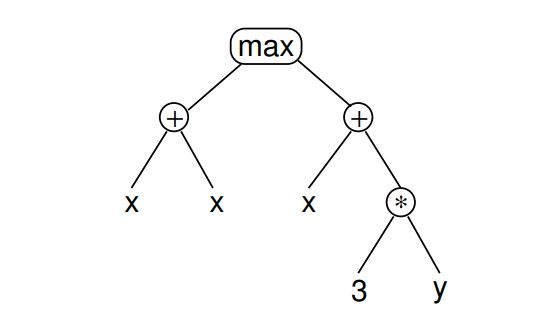
\includegraphics[width=0.5\linewidth]{fgtGP_tree}
	\caption{Sintaksno stablo (program) \cite{fieldguidtoGP}}
\end{figure}
 \par 
 Promjene su ključan dio razvoja programa, ali kao i u prirodi, promjene su nasumične i ne možemo garantirati da svaka promjena dovodi k boljem rješenju. Nasumičnost ima i svoje jače strane te često dovodi do novih i neočekivanih rješenja koja zaobilaze uobičajene poteškoće na koje nailaze determinističke metode \cite{fieldguidtoGP}. \par 
Prije uvođenja promjena vrši se selekcija. \textbf{Selekcija} je proces odabira roditelja uz pomoć kojih će se, kroz genetske operacije, uvesti novi programi u populaciju. U kasnijem poglavlju detaljnije ćemo opisati različite načine na koje se selekcija može izvesti. Bitno je da roditelji imaju veću šansu biti odabrani što su prilagođeniji našem zadatku. Osim toga, važno je dati mogućnost odabira manje prilagođenijih programa jer oni mogu sadržavati dijelove koji će dati bolje rezultate za generalni zadatak. 
\par 
Promjene između generacija događaju se zbog dvije ključne genetske operacije: 
\begin{itemize}
	\item \textbf{Križanje} (eng. \textit{Crossover}): Stvaranje novog programa/djeteta kombiniranjem nasumičnih dijelova roditeljskih programa
	\item \textbf{Mutacija} (eng. \textit{Mutation}): Stvaranje novog programa/djeteta nasumičnim mijenjanjem dijelova roditeljskog programa
\end{itemize}
\par
Oblik stabla čini križanje i mutaciju jednostavnijim i intuitivnijim. 
	\begin{figure}[h]
		\centering
		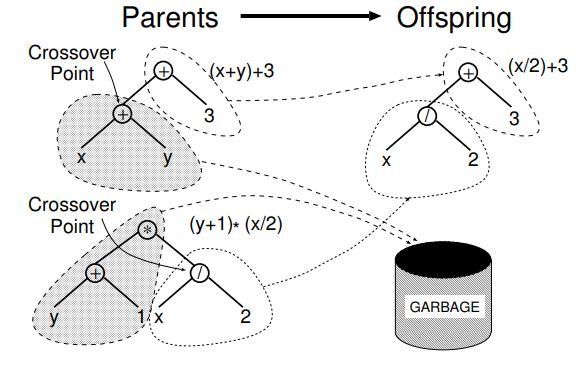
\includegraphics[width=0.7\linewidth]{fgtGP_crossover} 
		\caption{Križanje dviju kopija roditeljskih programa \cite{fieldguidtoGP}}
	\end{figure}
\newpage
\par
Križanje (Slika 3.2) možemo shvatiti kao miješanje i/ili zamjenu podstabala roditeljskih programa. Mutaciju (Slika 3.3) možemo shvatiti kao promjenu čvora gdje promjena može biti u obliku promjene funkcije/varijable na mjestu mutacije ili dodavanja u potpunosti novog podstabla na mjesto mutacije.\newline
	\begin{figure}[h]
		\centering
		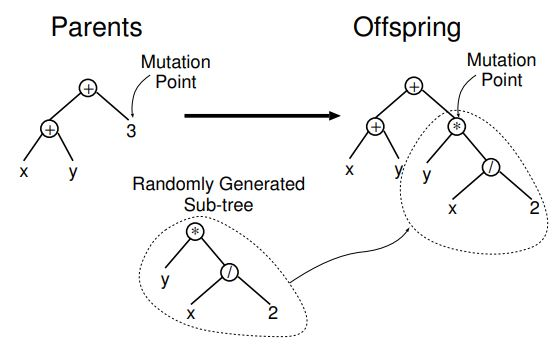
\includegraphics[width=0.7\linewidth]{fgtGP_mutation}
		\caption{Mutiranje roditelja dodavanjem novog podstabla na mjesto mutacije \cite{fieldguidtoGP}}
	\end{figure}
\par 
Napredak pojedinih programa prati se kroz generacije preko funkcije \textbf{dobrote}. \textbf{Dobrota} (eng. \textit{fitness}) je vrijednost koja ukazuje na to koliko je neki program dobar ili loš u rješavanju danog zadatka. Način računanja dobrote ovisni o tipu zadatka kojeg imamo te se prema tome može računati na različite načine.\par 
Dobrota nas dovodi do pojma elitizma u kojem ona igra glavnu ulogu. \textbf{Elitizam} je strategija kojom uspoređujemo dobrote programa unutar generacije te najbolji ili nekoliko najboljih programa trenutne generacije prebacujemo u sljedeću generaciju. Imamo veliku korist od ovakve strategije jer sprječava da najbolji program generacije bude lošiji od najboljih programa prošlih generacija. Sprječavamo nazadovanje kroz generacije.\par
Na kraju, mora postojati i \textbf{uvjet zaustavljanja} koji će reći da nema potrebe za daljnjim generacijama. \textbf{Uvjet zaustavljanja} može biti određena vrijednost dobrote ili dostizanje određenog broja generacija, ali može biti i neki drugi specifičan uvjet. 

	
